\documentclass[11pt,landscape]{article}
\usepackage[a3paper]{geometry}
\usepackage{graphicx}
\usepackage{fancyhdr}
\usepackage{multirow}
\usepackage{multicol}
\usepackage{textcomp}
\usepackage{gensymb}
\usepackage{amsmath, amssymb}
\usepackage{float}
\usepackage{wrapfig}
\usepackage{hyperref}
\usepackage[parfill]{parskip}
\usepackage{glossaries}
\usepackage{amsmath}
\usepackage{mdframed}
\usepackage{caption}
\usepackage{siunitx}
\geometry{margin=2.5cm}

\graphicspath{{./images/}}

\pagestyle{fancy}
\setlength{\headheight}{24pt}
\fancyhead[L]{GDP Group}
\fancyhead[R]{Design of Smart Autonomous Golf AGC}
\fancyfoot[C]{\thepage}


\title{GDP Draft Report}
\author{GDP Group}



\begin{document}
\pagenumbering{arabic}
\maketitle
\newpage
\begin{multicols}{3}
\tableofcontents
\newpage
\section{Introduction}
The main objective of the project was to design a smart and autonomous golf
caddy. A golf caddy is a person that carries a player’s golf bag and clubs and
gives the player advice and moral support. Our project consists in designing an
electronic trolley that can perform to its best the caddie’s job and help
players improve their golf game without having to pay a second person for their
service. This means being able to follow the player and suggest the optimal golf
club to choose in each shot. Although this idea has long been invented, we are
aiming to produce a prototype of a product that could stand out in the market.
Our competitive advantage over our rivals is our club release mechanism, which
releases the suggested club when needed and the fact that the caddy will not
follow the user if he or she enters the green or a hazard.

The improvement of the existing idea was proposed by James Siabi to our primary
supervisor Dr Mohamed Moshrefi-Torbati. James is our industrial supervisor who
after many years of playing golf and experiencing electronic golf trolleys,
found the gap in the market. Due to our lack of resources and time, the final
product consists in a prototype that will not be ready to commercialise but to
prove the possibility of a future commercialization.

\section{Design Brief}
\subsection{Project Aims}
At the beginning of the academic year the group decided on a set of aims to
achieve by the end of the project:

\begin{itemize}
    \item   Autonomously follow golfer
    \item   Automatically avoid hazard areas 
    \item   Suggest optimal club choice
    \item   Incorporate a mechanism to release suggested club
    \item   Incorporate a touchscreen display with a user interface
\end{itemize}

\subsection{Project objectives}
The objectives are more specific targets set to achieve the aims. These are:
\begin{itemize}
    \item	Enable real time GPS communication between pod and trolley
    \item	Design an algorithm to avoid obstacles in an efficient way
    \item	Learn golfer`s tendencies through a machine learning algorithm
    \item	Develop a light mechanism to release desired golf club
    \item	Design with Python a graphical user interface
\end{itemize}

\newpage
\end{multicols}
\section{Mechanical Design}
The final design of the AGC is shown in Fig. (\ref{fig:complete_design}).
\begin{figure}[H]
    \begin{center}
        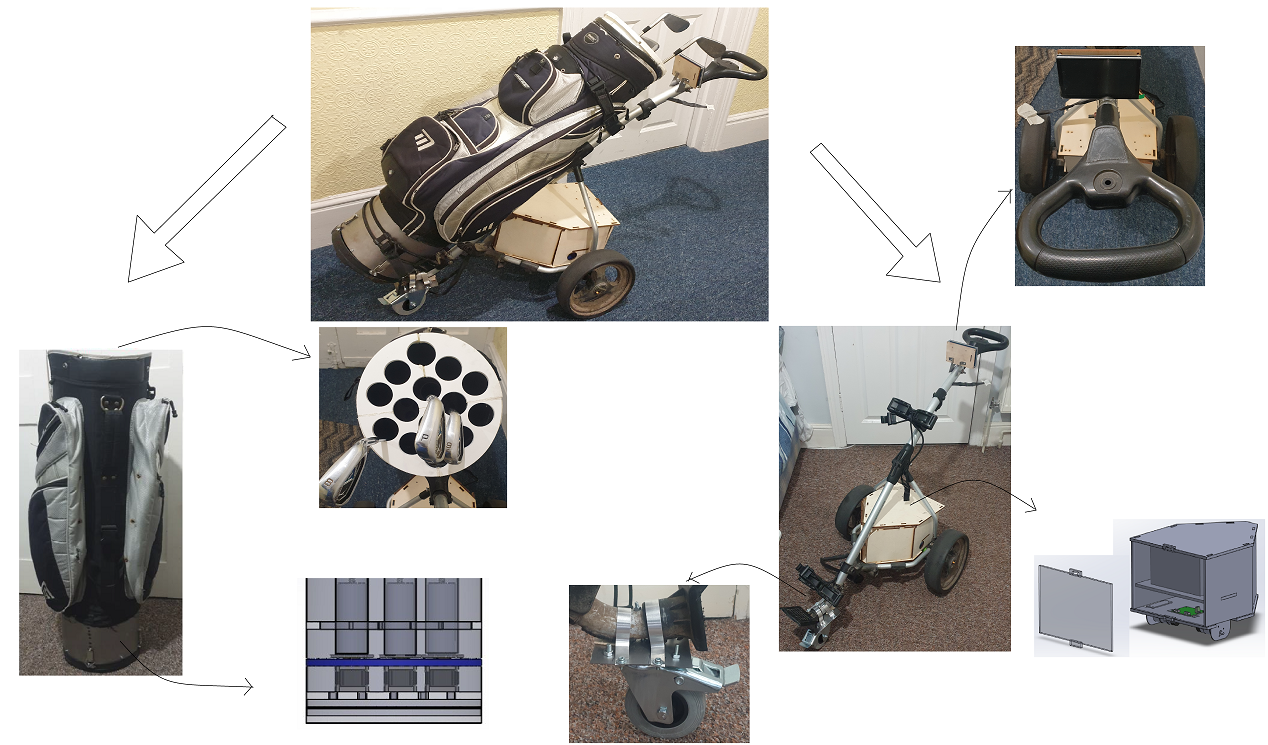
\includegraphics[width=\textwidth]{Complete Design.PNG}
        \captionof{figure}{Final AGC design}
        \label{fig:complete_design}
    \end{center}
\end{figure}

\newpage
\begin{multicols}{3}
\subsection{Club Raising Mechanism}
One of the key objectives for this project was to design and implement a release
mechanism that will give a golf club to the user based on its position on the
golf course and the distance to the green. This system will be used in
conjunction with the machine learning algorithm which will be the main brain
towards selecting which club to give to the user.

\subsubsection{Design Requirements}
\begin{itemize}
    \item Need to lift at least 10 cm above other golf club in order to make it
    clear which club is being given
    \item Needs to withstand the weight of the golf club which produces an axial loading
    \item Needs to be lightweight in order to not affect the entire golf bag
    since it will be carried by a user
    \item Needs to be a robust design since it will be used a lot of times
\end{itemize}

\subsubsection{Design Process}
Initially the team started discussing on the available workspace that can be
used to hold the mechanism. Two locations were identified, one was on the golf
AGC where the golf bag rests and the other being inside the golf bag itself.
The most feasible workspace was determined to be inside the golf bag since the
system on the golf AGC will have a higher probability of failing to work as it
would need to be aligned perfectly such that each mechanism is directly below
each golf club.

We then started investigating on possible configurations of systems that can
offer a linear motion that will push up the golf club. Some of the most
prominent ideas were to use linear actuators, slider-crank mechanism, an
umbrella like compression spring mechanism, and a stepper motor with a threaded
rod.

\paragraph{First Iteration}
After going through the various ideas presented, there were some clear
advantages and disadvantages with each of them. Starting with the linear
actuators, they are easy to use, robust in terms of mechanical functionality,
can be automated and be used in a controlled environment. However, they are
prone to be heavy in mass with one actuator weighing about 1.2kg.  If they were
to be used for 14 clubs, that would be an extra added weight of 16.8 kg which
will make the new golf bag, with the added actuators, 2.12 times heavier than
without them. This would be an issue for the golfer as they will have to carry a
bag over 30 kg, and it will also have an influence on the motors required to
drive the AGC since they will need provide more torque to propel forward.

For
the slider-crank mechanism, although it appears to be the simplest design to
adopt and use, the diameter of the crank would have had to be 10 cm if it is
required to elevate a golf club by 10 cm. Due to the restricted workspace
available in the golf bag to fit the mechanism, it would not be physically
possible to fit 14 cranks of diameter 10 cm in the golf bag. 

It now leads us to
the first feasible idea which is an umbrella like mechanism using compression
springs. Adopting a similar mechanism as in an umbrella, where a compression
spring is under compression and release due to the force input from a user, the
first design was built on CAD and is shown in Fig. (\ref{fig:init_release_mech}).
Fi. (\ref{fig:pin}) shows a 3D printed pin that will act similar to one found in an
umbrella.

\begin{figure}[H]
    \begin{center}
        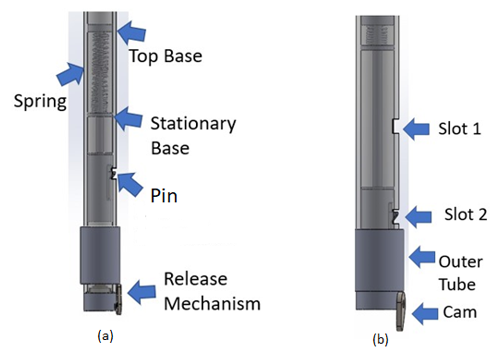
\includegraphics[width=0.3\textwidth]{Init Release Mech.PNG}
        \captionof{figure}{Mechanism in a) retracted state b) released state}
        \label{fig:init_release_mech}
    \end{center}
\end{figure}
\begin{figure}[H]
    \begin{center}
        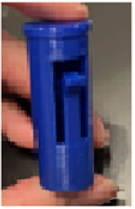
\includegraphics[width=0.1\textwidth]{pin.PNG}
        \captionof{figure}{Pin}
        \label{fig:pin}
    \end{center}
\end{figure}

In this design, a compression spring is attached to a moveable top base and
stationary base with a rod in the middle which leads to a pin that sits in
either slot 1, when the mechanism is in “released” state or slot 2, when the
mechanism is in “loaded” state. A user input is required to compress the spring
to make the mechanism enter the “loaded” state. In order to release the
compressed spring, which in turn gives the elevating effect, a stepper motor is
used with a cam attached to its axle. An outer tube rests on the cam and when
the cam rotates, the tube transfers its axial force received from the stepper
motor, tangentially to the pin, which then pushes the pin inside and releasing
the compressed spring. The pin will return to its original position once it
reaches slot 1 after it suffered an elastic deformation from the outer tube.

The mechanism was well suited for its purpose, however, the structural integrity
of the pin soon failed. Since it had to be 3D printed, due to its intricate
shape, the force acting on the pin acted as a cyclic loading which causes stress
induced cracking at the point of bending. This in turn made the pin to fracture
prematurely during testing. It was deemed that this design was too fragile to be
used for a prolonged amount of time as on a golf course.

This design was later improved due to the discovery of a mini electric lock that
has an inbuilt motor inside a door latch design. The mini electric lock and the
improved mechanism is shown in Fig. (\ref{fig:improv_release_mech}).

\begin{figure}[H]
    \begin{center}
        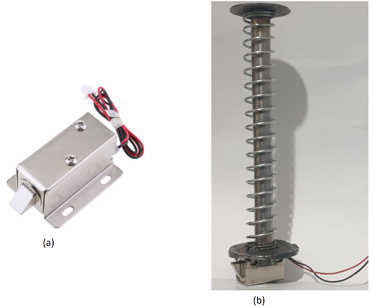
\includegraphics[width=0.3\textwidth]{Improv Release Mech.PNG}
        \captionof{figure}{a) Mini Electric Lock b) Improved Release Mechanism with electric lock}
        \label{fig:improv_release_mech}
    \end{center}
\end{figure}

The improvements on the original design made it more compact and rigid as a
mechanism. However, the electric lock did not perform well when it was in the
“loaded” state. The motor required a high torque and therefore a bigger size
lock would be needed. The overall dimensions of each electric lock would then
exceed the required amount in order to fit 14 in a golf bag for each club.
Moreover, since it is not a controlled release, safety issues may arise should
the mechanism release the golf club with excessive force which may hit the user.
This design as well was deemed not usable as a release mechanism.

\paragraph{Second Design Iteration}
Another innovative idea was to use a mechanism that employs a nut and bolt
analogy. If either a nut or bolt is fixed in free space and the other is
rotated, the only direction for motion is either up or down, depending on the
direction of rotation. Using this methodology, a stepper motor with a threaded
rod was used and a plate holder was attached to a nut that will sit on the
threaded rod of the stepper motor. This design was made to sit on the side of
the tube and by using the inner walls of the tube to prevent the rotation of the
nut, the only direction that the plate holder can move would be in the z-axis.
Fig. (\ref{fig:init_stepper}) shows how the setup of this design look
like. 

\begin{figure}[H]
    \begin{center}
        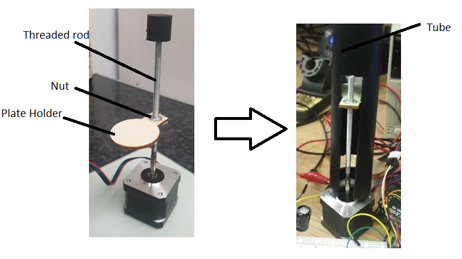
\includegraphics[width=0.3\textwidth]{Init stepper motor design.PNG}
        \captionof{figure}{Stepper motor with plate holder in tube}
        \label{fig:init_stepper}
    \end{center}
\end{figure}

Having weighted all the golf clubs given, the maximum mass recorded was around
700g. This mass was used in further calculation in order to obtain a required
torque to lift the club. Using a pulley analogy, for a mass of 700g being pulled
up at a radius, $r$. Eqs. (\ref{eq:raising_force} and \ref{eq:raising_torque}) 
can be used to calculate the force, $F$, and
torque, $T$, required to raise the club. Where $m$ is the mass of the club.
\begin{center}
    \begin{equation}
        F = W = mg_0
        \label{eq:raising_force}
    \end{equation}
\end{center}
\begin{center}
    \begin{equation}
        T = Fr
        \label{eq:raising_torque}
    \end{equation}
\end{center}The issues regarding this design were that the plate holder can get
stuck within the tube and therefore failing the whole system. Another issue was
that the pitch of the threaded rod was too close together which would mean that
the motor would have to rotate for a long amount of time to elevate the golf
club for 10 cm as required. This will decrease the overall operational lifespan
of the motor.

\paragraph{Final Design}
Finally, the mechanism that the team has opted for is a stepper motor with a
leadscrew alongside a 3D printed tube that will be elevated. Fig.
(\ref{fig:final_stepper}) shows the final design chosen for the release
mechanism.
\begin{figure}[H]
    \begin{center}
        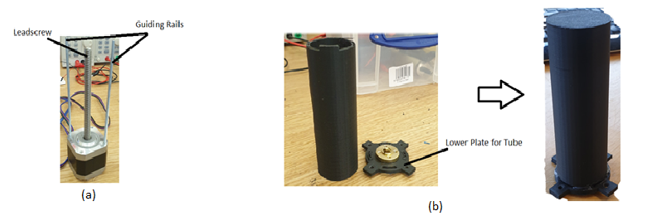
\includegraphics[width=0.3\textwidth]{Final Stepper motor design.PNG}
        \captionof{figure}{a) Stepper Motor with Leadscrew and guiding rails b) 3D Printed tube that sits on nut of leadscrew}
        \label{fig:final_stepper}
    \end{center}
\end{figure}

As the stepper motor shaft rotates, the tube that sits on the motor will try to
rotate as well. However, instead of using the inner walls of the tube to hold
the rotation, it now uses guiding rails prevent the rotation of the leadscrew’s
nut that is attached to the lower plate of the tube. Since there is a rotation
of the shaft and there is a restriction placed on the rotating movements, the
only direction of motion for the tube is either up or down.

The design chosen is more compact as it relies mostly on the operation of the
stepper motor and can be contained mostly in a small space. It also allows for a
more controlled release of the golf club and will have a high longevity since
stepper motors can last for a long time. The overall weight of this design only
amounts to 400g per mechanism and if it is to be used for 14 clubs in total,
that would be 5.6 kg added to a golf bag which in turn is about 37\% increase
from an original weight of 15 kg. Fig. (\ref{fig:stepper_in_bag}) shows how the mechanism
is set up inside in the golf bag.

\begin{figure}[H]
    \begin{center}
        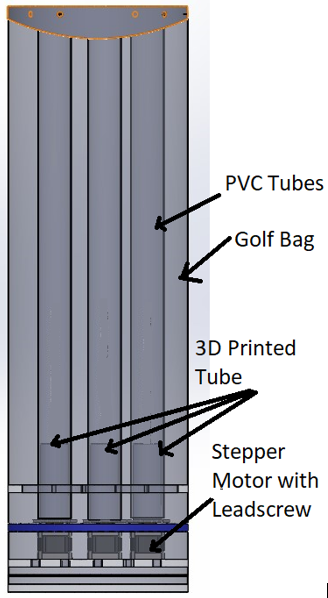
\includegraphics[width=0.3\textwidth]{Mech in bag.png}
        \captionof{figure}{Release Mechanism in golf bag}
        \label{fig:stepper_in_bag}
    \end{center}
\end{figure}

Table 1 lists the specification of the stepper motor used. This torque produced
is well enough within the required torque to raise the golf club even with a
factor of 3.

\begin{table}[H]
    \begin{center}
        \begin{tabular}{|l|l|}
            \hline
            \textbf{Parameter}     & \textbf{Value}          \\ \hline 
            Leadscrew Diameter     & $\SI{8}{\mm}$                  \\ \hline
            Leadscrew Length       & $\SI{150}{\mm}$ ($\pm\SI{1}{\mm}$)        \\ \hline
            Motor Dimensions       & $\SI{42}{\mm}\times\SI{42}{\mm}\times\SI{40}{\mm}$ (LxWxH) \\ \hline
            Step Angle             & $\SI{1.8}{\degree}$           \\ \hline
            Nut Material           & Brass                   \\ \hline
            Holding Torque         & $\SI{400}{\mN\m}$                \\ \hline
            Thrust (Full Step)     & $\SI{12.5}{\kg}$              \\ \hline
            Rated Current/Phase    & $\SI{1.5}{\ampere}$      \\ \hline
            Rated Voltage          & $\SI{3.3}{\volt}$     \\ \hline
            Rated Resistance/Phase &$\SI{2.2}{\ohm}\pm10$\%  \\ \hline
            Mass                   & $\SI{400}{\gram}$                  \\ \hline
        \end{tabular}
    \end{center}
    \captionof{table}{Stepper motor specifications}
\end{table}

\subsection{AGC Electrical Base}
\subsubsection{Design Requirements}
In order to control all the newly placed systems around the AGC, a base, that
will house all the electrical components and the battery, is required. The
design requirements for it are listed below.
\begin{itemize}
    \item Needs to hold all the components required for the AGC to operate
    the wheels, GPS module, Raspberry Pi, LCD Screen, and motors.
    \item Needs to be lightweight otherwise it increases the weight of the
    AGC which affect the motor size and power. 
    \item Needs to be easily accessible since the battery will be inside the
    casing and needs to be remove when charging is required.
    \item Needs to be waterproof and have a rigid structure such that the
    components do not move during movements on the golf course.
\end{itemize}
The most feasible place to have a base that will incorporate all the
requirements, is where the previous battery was located. After removing the
previous motors and battery plate holder, the new allocated space was measured
and built on CAD in order to design a new compartment. Fig.
(\ref{fig:prev_base}) shows the before and after replacing the previous motors
with the new electrical base.

\begin{figure}[H]
    \begin{center}
        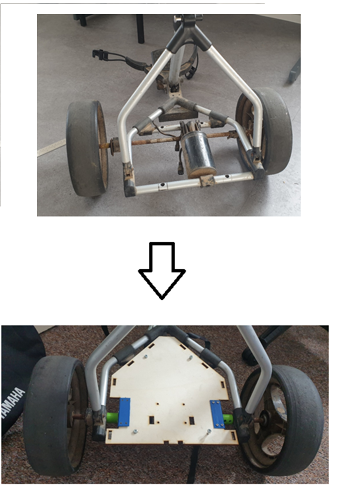
\includegraphics[width=0.3\textwidth]{Prev AGC base.png}
        \captionof{figure}{Replacing the previous AGC's motor with a base}
        \label{fig:prev_base}
    \end{center}
\end{figure}

\paragraph{Final Design}
Fig. (\ref{fig:new_base}) shows how the final base that will hold the
electronics and the battery looks like.
\begin{figure}[H]
    \begin{center}
        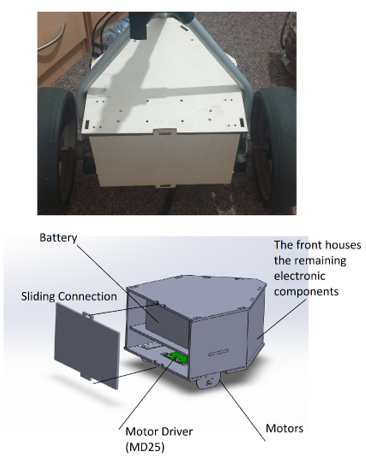
\includegraphics[width=0.3\textwidth]{New AGC base.PNG}
        \captionof{figure}{Full new AGC base}
        \label{fig:new_base}
    \end{center}
\end{figure}

\subsection{Wheels}
\subsubsection{Design Requirements}
The wheels of the AGC are one of the most important components that will
ensure a smooth and stable drive. They need to be able to give enough friction
and be able to adapt to the surface on a golf course. Since the AGC will have
to be autonomous and will need to be able to turn in certain events, a list of
new requirements for the wheels are listed below:

\begin{itemize}
    \item Maintain enough friction on wheels during acceleration such that it
    can be used on golf course
    \item Incorporate a system that allows the new motors chosen to operate one wheel individually
    \item Front wheels need to be able to turn 360 in order to accommodate when the rear wheels are made to make an arc using speed differentials between each wheel.
\end{itemize}

\paragraph{Design Process}
Initially the rear wheels on the original golf AGC were driven by a single
shaft as shown in Fig. (\ref{fig:prev_wheels}) and the front wheel was held in such a
way that allows movement only forward and backwards. 

\begin{figure}[H]
    \begin{center}
        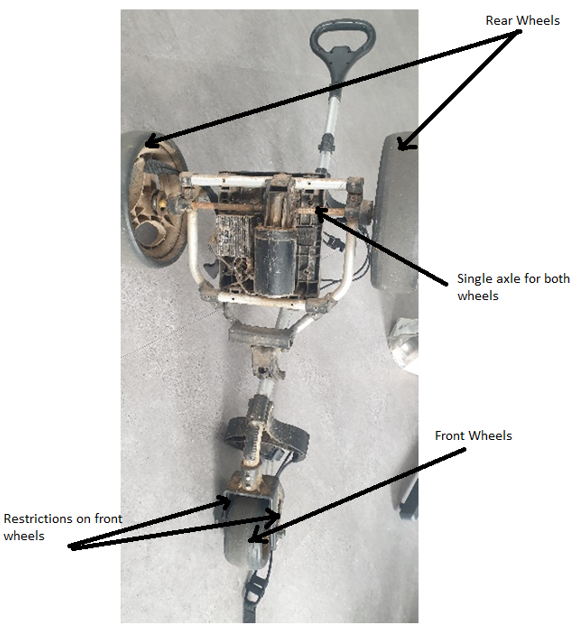
\includegraphics[width=0.3\textwidth]{Prev Wheels.PNG}
        \captionof{figure}{Previous wheels connection on original golf AGC}
        \label{fig:prev_wheels}
    \end{center}
\end{figure}


There were three options available to meet these design requirements. It was to
either design and manufacture our own wheels, to buy another readily available
wheel of the market, or to be more cost effective and re-use the current wheels.
The current rear wheels were on a single axle and therefore to make it
compatible to function with two separate motors, the shaft was cut down at two
separate locations. These locations were chosen since the wheel themselves
required a locking mechanism to the axle as shown in Fig. (\ref{fig:cut_axle}). In
order to not having to redesign the locking mechanism, it was best to cut
further down the axle such that it will be easier to join to the shaft of the
motors.

\begin{figure}[H]
    \begin{center}
        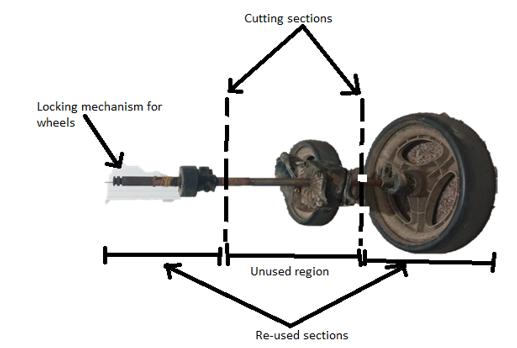
\includegraphics[width=0.3\textwidth]{Cut axle.PNG}
        \captionof{figure}{Single axle from previous golf AGC}
        \label{fig:cut_axle}
    \end{center}
\end{figure}

The wheels with the shaft attached and the shaft of the new motors were then
attached together with a shaft coupler. This shaft couple was designed, and 3D
printed with M2 holes that will go through each shaft and allow for a rigid
connection through the coupler. The shaft coupler 3D printed part is shown in
Fig. (\ref{fig:coupler}) and the connection between the wheels and motor is shown in
Fig. (\ref{fig:new_rear_wheels}).

\begin{figure}[H]
    \begin{center}
        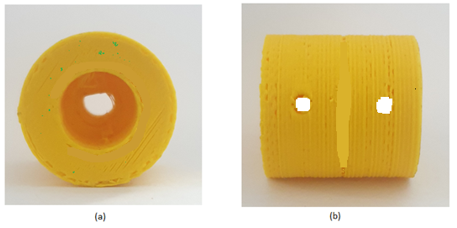
\includegraphics[width=0.3\textwidth]{coupler.PNG}
        \captionof{figure}{3D Printed Coupler to connect wheels and motor}
        \label{fig:coupler}
    \end{center}
\end{figure}
\begin{figure}[H]
    \begin{center}
        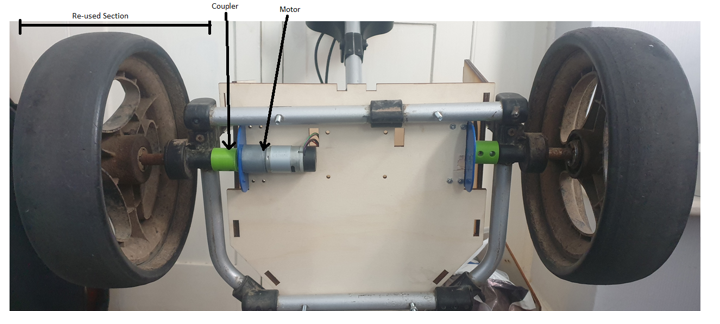
\includegraphics[width=0.3\textwidth]{New rear wheels.PNG}
        \captionof{figure}{New arrangement of motors and wheels with coupler}
        \label{fig:new_rear_wheels}
    \end{center}
\end{figure}
The next adjustment that needed to be done is the front wheel. The available
options we had were:
\begin{itemize}
    \item Design and manufacture a bracket which will hold the front wheel alongside a ball caster that allows for a full rotation of the wheel
    \item To buy a swivel castor wheel of the market
\end{itemize}

The team decided to go with the second option since the cost and reliability of
a ready-made swivel castor was better than a self-made one. The selected swivel
castor is shown in Fig. (\ref{fig:castor}).

\begin{figure}[H]
    \begin{center}
        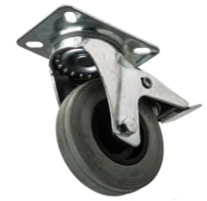
\includegraphics[width=0.3\textwidth]{Swivel castor.PNG}
        \captionof{figure}{Swivel Castor Wheel}
        \label{fig:castor}
    \end{center}
\end{figure}

Since the original location of the attachment of the wheels is not horizontal,
the new swivel castor wheel could not rotate properly since it was at angle.
Therefore, a sheet metal was attached at the uttermost low point of the AGC's
main frame for the front wheel and then the wheel was attached to it. Fig.
(\ref{fig:new_front_wheels}) shows how the previous wheel and the new swivel
caster wheel are attached to the golf AGC.

\begin{figure}[H]
    \begin{center}
        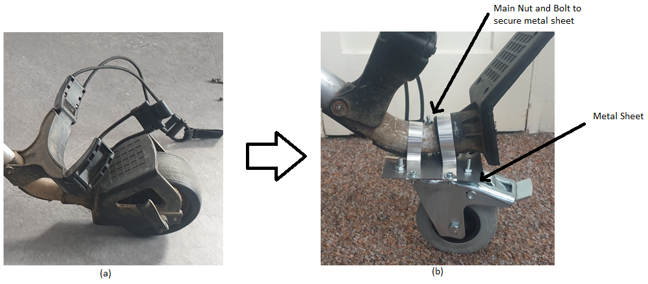
\includegraphics[width=0.3\textwidth]{New front wheels.PNG}
        \captionof{figure}{a) Initial front wheel connection b) Swivel castor wheel attached to metal sheet}
        \label{fig:new_front_wheels}
    \end{center}
\end{figure}

\paragraph{Final Design}
Fig. (\ref{fig:final_wheels}) shows how the AGC looks like after assembling
all the wheels.

\begin{figure}[H]
    \begin{center}
        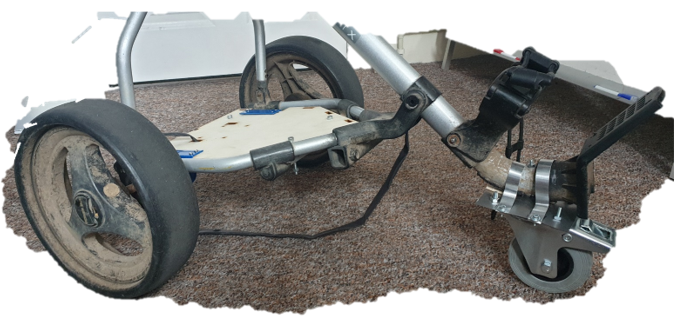
\includegraphics[width=0.3\textwidth]{Full wheels.PNG}
        \captionof{figure}{Complete assembly of golf AGC with new wheels connection}
        \label{fig:final_wheels}
    \end{center}
\end{figure}


\section{Software}
\label{software}
In this section all software required for the operating cycle of the AGC is
discussed. The AGC main computer is a Raspberry Pi 4 running a 64-bit Debian port,
the same is true for the Raspberry Pi used in the tracking pod. The GPS
navigation system requires high precision decimal storage to operate properly.
Data type \verb|float32| can store 23 significant bits, compared to data type
\verb|float64| which can store 52 significant
bits\cite{floating_point_goldberg}. 
The calulcations shown below in Fig. (\ref{fig:float_calcs}) show the
physical significance of which datatype is chosen.
\begin{figure}[H]
    \begin{mdframed}
        Only $180^{\circ}$ need to be accounted for because sign bit is separate, so to
        represent $180^{\circ}$ the bits required is:
        \begin{center}
            \begin{equation*}
                \log_2{180} \approx 7.49185 bits
            \end{equation*}
        \end{center}
        This leaves the $n - 7.49185$ significant bits left for sub degree
        representation, the physical precision in meters we can then derive from each
        data type of a longitude value at the equator can be calculated as shown in
        the equations below.\newline
        \begin{center}
            \begin{minipage}{0.45\textwidth}
                \begin{mdframed}
                    For \verb|float32| $n=23$:
                    \begin{center}
                        \begin{equation*}
                            \frac{\frac{R_e \cdot \pi}{180}}{2^{\left(52 - \log_2{180}\right)}} \approx 2.386m
                            \label{eq}
                        \end{equation*}
                    \end{center}
                \end{mdframed}
                \end{minipage}
                \begin{minipage}{0.45\textwidth}
                    \begin{mdframed}
                For \verb|float64| $n=52$:
                \begin{center}
                    \begin{equation*}
                        \frac{\frac{R_e \cdot \pi}{180}}{2^{\left(52 - \log_2{180}\right)}} \approx 4.44nm
                    \end{equation*}
                \end{center}
            \end{mdframed}
            \end{minipage}
        \end{center}
        \center The radius of Earth. $R_e$, value used was $6371000m$. 
    \end{mdframed} 
    \captionof{figure}{Calculations showing physics precision of single vs double
    precision floats}
    \label{fig:float_calcs}
\end{figure}
The $180^{\circ}$ is normalised to a power of two so we are able to use the non
integer value of bits in the calculation for physical precision, were we to not
perform this normalisation then $7.4918\rightarrow8$ full bits are required to
represent the degrees and the final
precision is slightly less for each datatype. To ensure this calculated
precision is representative of our system all GPS coordinates are normalised to
a power of two. We can see from the calculations that a significantly higher
precision is achieved using double precision floating point data type to store
GPS values. The precision yielded by the double precision floating point is
unnecessary, however the precision of the single precision floating point is too
low as our GPS module is capable of providing more accurate GPS measurements as
discussed in section \ref{electronics}. Therefore double precision floating
point datatypes will be used to store GPS data, which requires us to use a
64-bit compatible operating system which is why the 64-bit Debian port was
chosen. The higher precision achieved comes at the cost of slightly higher
compte time for calculations, however as most of the algorithms onboard operate
only on small amounts of data, this effect is unnoticable when operating the
AGC.

\subsection{Control Software}
\label{control_software}
This section discusses the software used to make the AGC follow the golfer.
All of the control software apart from the elctronics specific code, such as
motor controller communication, was written first using the OpenGL simulator
that was built throughout the year. Building and using a simulator allowed us to 
write and test all the control software / algorithms that would be required to make 
the AGC follow the golfer as intended while avoiding hazard regions.

All of the control software tested in the simulator was written in C as this was
easiest to use with OpenGL, however we decided to change to PyQt5 for designing
the onboard GUI. As the ACG software was now to be written in Python the control
algorithms were re-written in Python, however upon testing it was found that
their performance was significantly slower than the C implementations. This is
most likely a large number of array passing and manipulations are required,
which is significantly slower in Python where function arguments are passed as
object reference instead of pointers in C. Therefore the original C control
algorithms were compiled as a dynamic link library (DLL) and the Python ``C
Types'' library was used to load the DLL and create Python wrappers for the control
algorithms. This significantly improved the performance as all of the resource
intensive calculations were now performed with a compiled C program.

The main control loop that determines the AGC's behaviour is shown below in
Fig. (\ref{fig:control_loop}).
\begin{figure}[H]
\begin{mdframed}
    \begin{center}
        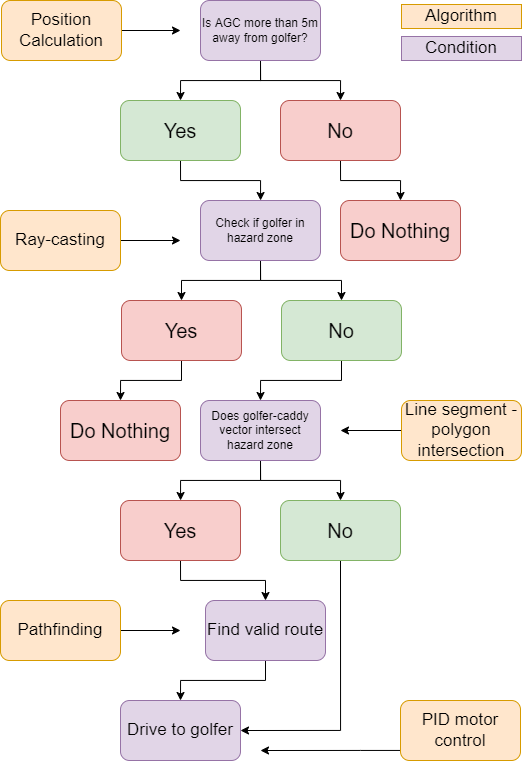
\includegraphics[width=0.9\textwidth]{control_loop.png}
    \end{center}
\end{mdframed}
\captionof{figure}{Main AGC control loop}
\label{fig:control_loop}
\end{figure}
\subsubsection{Map Processing}
As discussed in the introduction to section \ref{software}, all GPS
coordinates are normalised to a power of two. We also ``pad'' the hazard zone
coordinates, before normalisation, by a safety factor of two meters, preventing innacurate GPS
readings or hazard zone coordinates resulting in the AGC entering a hazard zone.
We ``pad'' the hazard zones by calculating the coordinates of centroid of the
polygon, then extending the vector from the centroid to each perimeter point by
two meters. The centroid of a polygon can be calculated from the coordinates of
it's perimeter points as shown in Eqs. (\ref{eq:cx} and \ref{eq:cy}).
\begin{center}
    \begin{equation*}
        A=\frac{1}{2}\sum_{i=0}^{n-1}\left( x_i y_{i+1} - x_{i+1} y_i\right)
    \end{equation*}
\end{center}
\begin{center}
    \begin{equation}
        C_x=\frac{1}{6A}\sum_{i=0}^{n-1} (x_i + x_{i+1}) (x_i y_{i+1} - x_{i+1} y_i)
        \label{eq:cx}
    \end{equation}
\end{center}
\begin{center}
    \begin{equation}
        C_y=\frac{1}{6A}\sum_{i=0}^{n-1} (y_i + y_{i+1}) (x_i y_{i+1} - x_{i+1} y_i)
        \label{eq:cy}
    \end{equation}
\end{center}
\subsubsection{Ray Casting}
The ray casting algorithm is used to determine whether a point falls within a
polygon. The algorithm can only accept polygons with straight edges; our polygons are
represented by a series of GPS points along their perimeter, and so our polygons
are defined by a series of small straight edges. The concept of this algorithm
is that given a point you wish to test, if you cast a ray from the point in one
direction to infinity, the number of intersections the ray has with the polygon
in question indicates whether the point falls in the polygon or not. If an even
number of intersections are found, then the point lies outside the polygon, and
if an odd number of intersections are found the point lies within the polygon.
A visual of this concept can be seen below in Fig. (\ref{fig:raycasting}).
\begin{figure}[H]
    \begin{mdframed}
        \begin{center}
            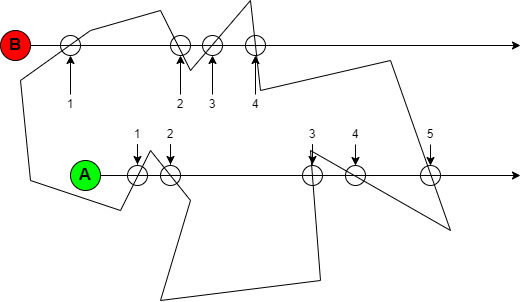
\includegraphics[width=0.95\textwidth]{raycasting.png}
        \end{center}
    \end{mdframed}
    \captionof{figure}{Raycasting Example}
    \label{fig:raycasting}
\end{figure}

The figure shows two points which are to be tested to determine if they lie
within the polygon. Casting the ray to the right, towards $x\rightarrow\inf$ in
our implementation, we can count the intersections each ray has with the
polygon. Point A has five intersections and so lies outside the polygon, point B
has four intersections and lies within the polygon. 

There are additional considerations in our implementation to accout for the ray
intersecting a vertex or for the ray being collinear with a polygon edge. If a
vertex is intersected then two intersections are counted, one for each edge
forming the vertex, and the result is not affected. If the ray is collinear
with a polygon edge then only a single intersection is counted, but the ray will
undoubtedly also intersect at least one of the vertices on the collinear edge
which will be appropriately accounted for.
The algorithm has been tested and does not fail in either of these cases.

\subsubsection{Segment Polygon Intersection}
Before the AGC starts moving towards any target destination, it first checks
that it's intended translation vector joining it's location to the target
location does not pass through
any hazard zones. It does this by checking that it's intended translation vector
doesn't intersect any edges of polygons. The diagram shown below in Fig.
(\ref{fig:segment_intersection}) depicts two finite length line segments
intersecting.
\begin{figure}[H]
    \begin{mdframed}
        \begin{center}
            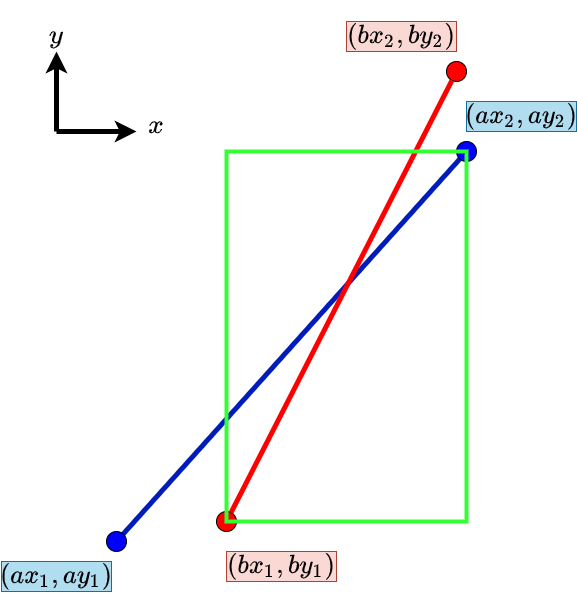
\includegraphics[width=0.95\textwidth]{segment_intersection.png}
        \end{center}
    \end{mdframed}
    \captionof{figure}{Line Segment Intersection Diagram}
    \label{fig:segment_intersection}
\end{figure}
 
The edges of polygons are defined only by the positions of two vertices, as is
the AGC intended translation vector. To calculate where the intersection point
of these two line segments are a mathematical equation for a line must be
constructed for each segment as shown in Eqs. (\ref{eq:line_a} and
\ref{eq:line_b}) respectively, then these equations can be solved simultaneously
to determine the location of the intersection as shown in Fig.
(\ref{fig:segment_calculations}).

After the intersection point is calculated we ensure that the intersection point
falls within the smallest rectangle bounded by one point from the first and
second coordinates of either segment. We do this because the equation for a line is infinite, and
any lines with non equal gradient will intersect, but we are only interested if
the intersection occurs between points the AGC intends to travel. The bounding
rectangle is demonstrated by the green rectangle in Fig. (\ref{fig:segment_intersection}).

\begin{figure}[H]
    \begin{mdframed}
        \begin{center}
            \begin{equation}
                ay_1-y = \frac{ay_2 - ay_1}{ax_2 - ax_1} \times (x - ax_1)
                \label{eq:line_a}
            \end{equation}
            \begin{equation}
                by_1-y = \frac{by_2 - by_1}{bx_2 - bx_1} \times (x - bx_1)
                \label{eq:line_b}
            \end{equation}
        \end{center}
    In our implementation, before this system is solved, we check
    if the lines have equal gradient, and if they are collinear or not. If they
    have equal graident, defined by:
    \begin{center}
        \begin{equation*}
            \frac{ay_2 - ay_1}{ax_2 - ax_1} = \frac{by_2 - by_1}{bx_2 - bx_1}
        \end{equation*}
    \end{center}
    Then we check if they are collinear, defined by:
    \begin{center}
        \begin{equation*}
            (x - ax_1) = (x - bx_1)
        \end{equation*}
    \end{center}
    If they are collinear then they intersect, if the have equal gradient but
    are not collinear then they do not intersect. If one or both of the lines
    are vertical, $(y_1 = y_2)$ then the system is not solved as below but
    trivially using the $x$ position of the line.\vspace{0.5cm}
    \newline
    For simplification:
    \begin{center}
        \begin{equation*}
            m_a = \frac{ay_2 - ay_1}{ax_2 - ax_1} \hspace{1cm} m_b = \frac{by_2 - by_1}{bx_2 - bx_1}
        \end{equation*}
    \end{center}
    Now we solve the system defined by Eqs. (\ref{eq:line_a} and
    \ref{eq:line_b}) to determine the point of intersection resulting in the $x$
    coordinate given by Eq. (\ref{eq:x}) and $y$ coordinate given by Eq. (\ref{eq:y}).
    \begin{center}
        \begin{equation}
            x = \frac{ax_{1} m_{a} - ay_{1} - bx_{1} m_{b} + by_{1}}{m_{a} - m_{b}}
            \label{eq:x}
        \end{equation}
        \begin{equation}
            y = \frac{ax_{1} m_{a} m_{b} - ay_{1} m_{b} - bx_{1} m_{a} m_{b} + by_{1} m_{a}}{m_{a} - m_{b}}
            \label{eq:y}
        \end{equation}
    \end{center}
    \end{mdframed}
    \captionof{figure}{Calculation of Line Segment Intersection Point}
    \label{fig:segment_calculations}
\end{figure}

\subsubsection{Pathfinding}
The pathfinding algorithm is only used if the control loop shown in Fig.
(\ref{fig:control_loop}) determines that the AGC should move to the golfer but
the a direct route is not possible due to the presence of a hazard zone between
them. Initially the A* pathfinding algorithm was researched as it is a well known algorithm
with which we could choose some heuristic function to minimise, in our case that
heuristic function would likely be the shortest distance to reach the golfer.
 A* is generally used
for pathfinding on a discrete graph, we do not have a discrete graph
available and so would have to construct one for each golf course or a local graph
surrounding the hazard we wish to avoid. This adds unnecessary complexity in
terms of implementation and computation to our system which we wish to avoid.
Additionally, A* has time complexity of $O(b^d)$ if $d$ is the shortest path length
and b is the branching factor, and the algorithm has high memory requirements as all generated
nodes are kept in memory \cite{astar_2009}. It
was decided we would not use A* algorithm. The next consideration was to simply
``pad'' the perimeter of the hazard polygon and follow it all the way around
until the AGC reaches the golfer. This concept is shown in
the diagram below in Fig. (\ref{fig:padding}) where the red line denotes
the path that would be taken by the AGC to avoid a hazard zone. Clearly this is
an inefficient path the AGC will unnecessarily follow the contour of the
polygon. Additionally, this method increases the risk that the AGC enters the
hazard zone if our GPS system is not performing well, or if our GPS mapping of
hazard zones is erronous.  


\begin{figure}[H]
    \begin{mdframed}
        \begin{center}
            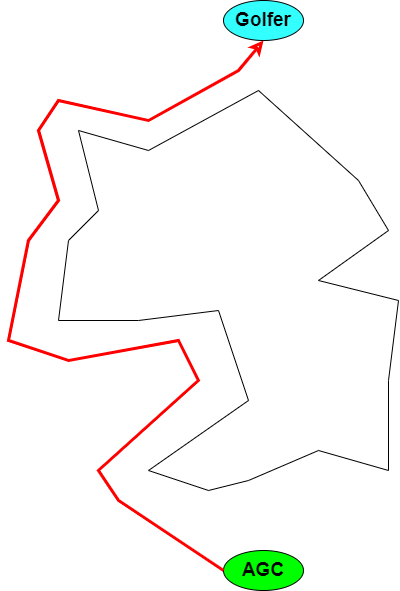
\includegraphics[width=0.95\textwidth]{padding.png}
        \end{center}
    \end{mdframed}
    \captionof{figure}{Path derived by ``padding'' polygon}
    \label{fig:padding}
\end{figure}

A custom pathfinding algorithm was designed and implemented. The path it finds
is not the optimal solution, but it computes quickly and the path derived is
more efficient than using the ``padding'' method. Fig.
(\ref{fig:pathfinding_flow}) shows the main steps performed by the algorithm to
determine where the AGC should go.

\begin{figure}[H]
    \begin{mdframed}
        \begin{center}
            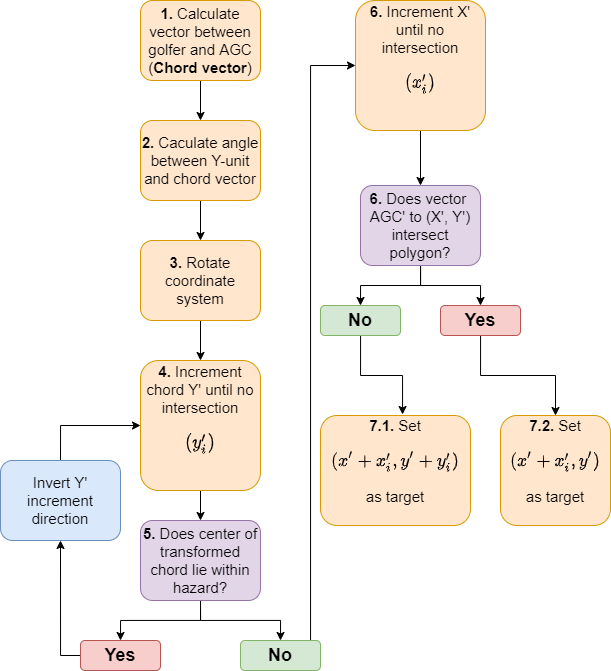
\includegraphics[width=0.95\textwidth]{pathfinding_flow.png}
        \end{center}
    \end{mdframed}
    \captionof{figure}{Pathfinding algorithm main steps}
    \label{fig:pathfinding_flow}
\end{figure}

First the chord vector, $\overrightarrow{\mathbf{C}}$, is calculated, along with
the angle, $\theta$, between $\overrightarrow{\mathbf{C}}$ and the Y-unit vector,
$\hat{\mathbf{y}}$, using Eq. ().  The relevant polygon, golfer position, and AGC
position are rotated about the z-axis with the center of rotation as the
origin by $\theta$ using Eq. () where $\overrightarrow{p}$ is a
three dimensional point and $\overrightarrow{p^\prime}$ is the rotated point. 
The polygon is rotated by applying Eq. () to each
vertex. The purpose of the rotation was to aid the design process of the
algorithm and make the code more readable, removing the necesscity for vector
manipulations throuhout the algorithm instead using only simple arithmetic operations.
This results in $\overrightarrow{\mathbf{C}^\prime}$ having constant $y$. The
value of $y^\prime$ is increment in one meter steps until no intersection
between the translated chord vector, $\overrightarrow{\mathbf{C}^\prime_t}$, and
the rotated polygon, $\mathbf{P}^\prime$. If any point of
$\overrightarrow{\mathbf{C}^\prime_t}$ lies within the polygon the increment
direction is reversed and incremented until there is no intersection and no
points of $\overrightarrow{\mathbf{C}^\prime_t}$ lie within the polygon. This
increment process is repeated in the $x^\prime$ direction for the vector joining
the rotated AGC position,
$\left(x^\prime_{AGC}, y^\prime_{AGC}\right)$, to $\left(x^\prime_{AGC},
y^\prime_{AGC} + y^\prime_i\right)$. Once the incrementation process if finished
such that no intersections are found, the vector joining $\left(x^\prime_{AGC},
y^\prime_{AGC}\right)$ to $\left(x^\prime_{AGC}+x^\prime_i,
y^\prime_{AGC} + y^\prime_i\right)$ is checked for intersections. If none are
found then $\left(x^\prime_{AGC}+x^\prime_i,
y^\prime_{AGC} + y^\prime_i\right)$ is rotated back to the original coordinate
system and set as the position target for the AGC. If an intersection is found
then $\left(x^\prime_{AGC}+x^\prime_i, y^\prime_{AGC}\right)$ is rotated back to
the original coordinate system and set as the AGC position target. This process
repeats until the golfer is reached. Incrementing in the $y^\prime$ direction
is equivelant to incrementing perpendicular to
$\overrightarrow{\mathbf{C}}$ in
the original coordinate system, and incrementing it by $x^\prime$ is equivelant
to incrementing in the direction of $\overrightarrow{\mathbf{C}}$.
\subsubsection{Pathfinding Diagram}
Fig. (\ref{fig:pathfinding_visual}) shows a visual of how the pathfinding algorithm will determine intermediary
positions for the AGC to move it towards the golfer. For the generation of this
figure the pathfinding algorithm was only called again after the target position
is reached, resulting in the very wide path that can be seen in the final path
diagram. On the AGC the pathfinding algorithm is called every time new GPS data
is available, approximately every second, resulting in a smoother and closer
path being found.
\end{multicols}
\newpage
\begin{figure}[H]
    \begin{mdframed}
        \begin{center}
            \begin{minipage}{0.3\textwidth}
                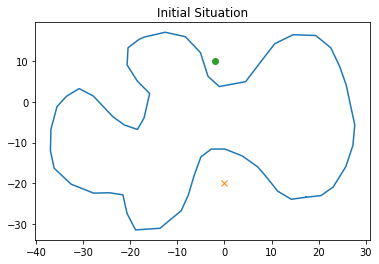
\includegraphics[width=0.95\textwidth]{initial.png}
            \end{minipage}
            \begin{minipage}{0.3\textwidth}
                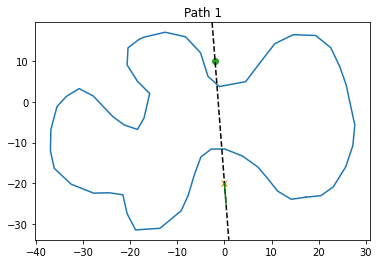
\includegraphics[width=0.95\textwidth]{p1.png}
            \end{minipage}
            \begin{minipage}{0.3\textwidth}
                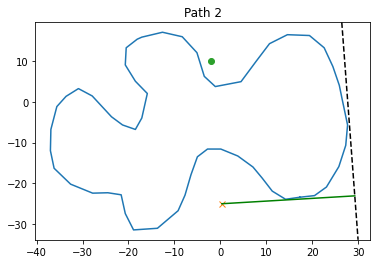
\includegraphics[width=0.95\textwidth]{p2.png}
            \end{minipage}
        \end{center}
        \begin{center}
            \begin{minipage}{0.3\textwidth}
                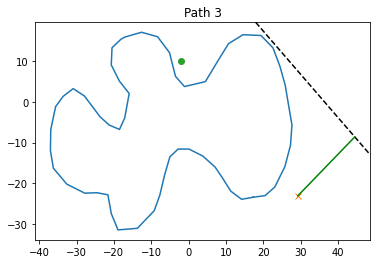
\includegraphics[width=0.95\textwidth]{p3.png}
            \end{minipage}
            \begin{minipage}{0.3\textwidth}
                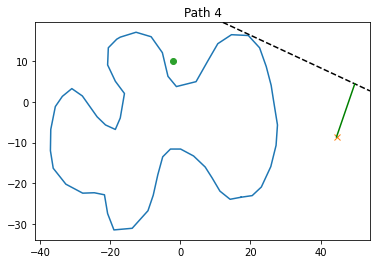
\includegraphics[width=0.95\textwidth]{p4.png}
            \end{minipage}
            \begin{minipage}{0.3\textwidth}
                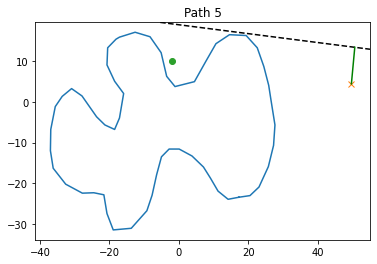
\includegraphics[width=0.95\textwidth]{p5.png}
            \end{minipage}
        \end{center}
        \begin{center}
            \begin{minipage}{0.3\textwidth}
                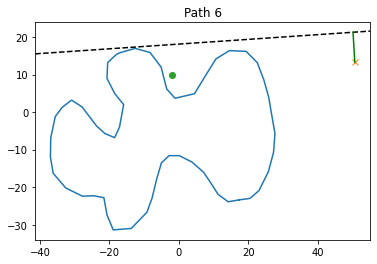
\includegraphics[width=0.95\textwidth]{p6.png}
            \end{minipage}
            \begin{minipage}{0.3\textwidth}
                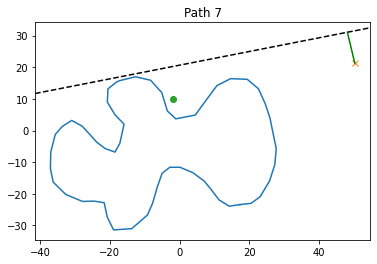
\includegraphics[width=0.95\textwidth]{p7.png}
            \end{minipage}
            \begin{minipage}{0.3\textwidth}
                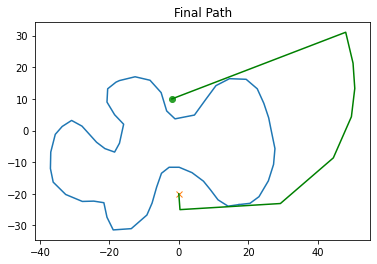
\includegraphics[width=0.95\textwidth]{final.png}
            \end{minipage}
        \end{center}
    \end{mdframed}
    \captionof{figure}{Visualisation of path determined by pathfinding algorithm}
    \label{fig:pathfinding_visual}
\end{figure}
\newpage

\begin{multicols}{3}

\subsection{Communications}
The EMG30 motors we are using are controlled by the MD25 motor controller board
via and $I^2C$ interface. The communication interface for this was written in C
and is capable of handling multiple $I^2C$ devices. Currently the only device we
have on the communications network is the MD25. The GPS in the golfer's pod communicates to the main Raspberry Pi via Bluetooth,
which is written in Python using the PyBluez library. The GPSs communicate with
the Raspberry Pis via serial commuication implemented using the Pyserial
library.

\subsection{GCP Elevation API}
The elevation is needed because the height difference in golf shots is relevant
to decide the optimal club choice. Hence, the first idea was to use a Google
Cloud Platform (GCP) elevation application programming interface (API). The
platform allows a free trial period and after this the price per 1000 request is
of 4-5 USD. 

Having the location of the pod, which will be carried by the user, and the
location of the hole in the golf course, the height difference can be known by
transforming the location into latitude and longitude coordinates.


\subsection{GUI}
\subsubsection{Course Map}
The course map was implemented on the GUI using the map system that was used on
the simulator. We attempted to embed a map web app called folium which looks
better than the map developed for the simulator, however, it doesn't allow us to
retreive coordinates for a point clicked on the map in real latitude / longitude
coordinates or in screen coordinates. This shortfall makes it impossible to give
the golfer the ability to click a point on the map and see how far away it is
from the AGC, using the simulator map allows us to add that feature.

\section{Machine Learning}
The AGC will have the option to enable optimal club choice predictions if the
user desires it. This option is placed on the AGC because current golf
regulations outside the United States do not permit the use of software to help
the golfer.

To determine the appropriate machine learning algorithm we first look at the
type of data we have. The AGC will collect both input and output data. Input
data will be mainly personal information from the user and type of club chosen
while output data will be the result of those chosen parameters. Hence, the
model uses supervised learning. From supervised learning we can do a regression
or classification model. The latter one is most suitable because we are
predicting labels and not quantities.


\section{Electronics}
\label{electronics}
\subsection{Motors}
The motors we decided to use for our prototype version are the EMG30 motors
because we already have them and this will save cost. However, they are
underpowered as they will take too long to accelerate the AGC to full speed, and
won't work at on anything more than a slight incline; for a final version the
EMG49 motors should be used. 
We chose these motors
by
considering the top speed we wish the AGC to able to go, and how fast we want it
to accelerate to that speed on a $10^\circ$ incline. The calculations shown below in
Fig. (\ref{fig:motor_calcs}) show how we calculated the necessary toruqe and rpm we require from our
motors.

\begin{figure}[H]
    \begin{mdframed}
        The top speed we chose for the AGC was 5.0 kilometers per hour,
        equivalent to average walking speed. 
        The wheel radius, $W_r$ of the AGC wheels is 0.115 meters. We can
        calculate RPM using Eq. (\ref{eq:rpm}):
        \begin{center}
            \begin{equation}
                rpm = \frac{7.5 * \frac{1000}{3600}}{2\pi W_r} \cdot 60 \approx 115rpm
                \label{eq:rpm}
            \end{equation}
        \end{center}
        The AGC should be able
        to accelerate to this speed, $V$, within $t=5$ seconds on a $10^\circ$ incline.
        For predicted final mass, $M = 15kg$, 
        the accelerating force, $F$, required can be calculated with Eq. (\ref{eq:accel}):
        \begin{center}
            \begin{equation}
                F = \frac{V}{t} + M g_0 \sin(10^\circ)\approx 29 N
                \label{eq:accel}
            \end{equation}
        \end{center}
        Finally the torque required from each motor can bel calulated using Eq.
        (\ref{eq:torque}):
        \begin{center}
            \begin{equation}
                T = W_r * F \approx 1.7 Nm
                \label{eq:torque} 
            \end{equation}
        \end{center}
    \end{mdframed}
    \captionof{figure}{Motor requirement calculations}
    \label{fig:motor_calcs}
\end{figure}

According to their datasheet the EMG49 motors can provided a loaded rpm of 122
and a torque of 1.56, close to our requirements set out above. As the torque is
slightly lower than calulated, the AGC will accelerate slightly to top speed on
a $10^\circ$ incline in slightly over five seconds.

\subsection{Power Supply}
The power for the trolley will be supplied by a 12v XXXXmAh LiPo battery. The
battery will be splitting 12v to the stepper and DC motors and 5v to the
microcontroller. Hence, the need of a 5v voltage regulator, provided by the
university, between the raspberry pi and the battery. The battery was supplied
by our project sponsor for free, so it is not included in the budget. The
battery output connector was cut and the copper wires were introduced into a
2-pin screw terminal with an insulated and heat-shrinked plastic tube.


\subsection{Touchscreen Display}
The touchscreen used is a 5 inch DSI capacitive touch display. It was chosen
because of its simple connection to the raspberry pi, which only consist of a
ribbon, and its affordable offer. It also brings mounting holes and screws to
fit it in a case as we have done in the AGC shown in fig X. 

\newpage
\nocite{*}
\bibliographystyle{ieeetr}
\bibliography{./ref}
\end{multicols}



\end{document}